% Python 画图
% Python|画图|matplotlib|标题|坐标轴

\subsection{python绘图库 matplotlib 的使用}

python绘图有很多库, 其中matplotlib库是最受欢迎的绘图库.如果熟悉 Matlab\upref{Matlab} 软件的用户,对matplotlib库就很容易上手,因为matplotlib中很多命令命名与用法与matlab十分类似. 首先在使用之前需要导入模块,并取别名plt.
\begin{lstlisting}[language=python]
import matplotlib.pyplot as plt
\end{lstlisting}
如果使用jupter等在线编辑器,一般需要加入
\begin{lstlisting}[language=python]
% matplotlib inline
\end{lstlisting}
来告诉解释器在浏览器中显示图像.现在我们来看看如何使用这个库.例如在 [0,5] 区间均匀取30个点,分别计算$\sin(x)$与$\exp(x)$,并作图
\begin{lstlisting}[language=python]
A = np.linspace(0,5,30) 
B = np.sin(A)
C = np.exp(-A)
plt.plot(A,B)
plt.hold(True)
plt.plot(A,C)
\end{lstlisting}
上述代码通过 \verb|hold| 把两个图像放在一张画布上面, 如\autoref{PyPlot_fig1} 所示.
\begin{figure}[ht]
\centering
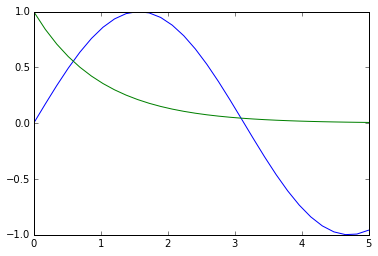
\includegraphics[width=9cm]{./figures/PyPlot_1.png}
\caption{$\sin(x)$与$\exp{x}$} \label{PyPlot_fig1}
\end{figure}


下面给一个综合案例来详细说明这个库的具体使用.结果如\autoref{PyPlot_fig2} 所示.
\begin{lstlisting}[language=python]
import matplotlib.pyplot as plt
import numpy as np
import matplotlib as mpl

mpl.rcParams["font.sans-serif"]=['kaiti']
mpl.rcParams['axes.unicode_minus']=False
plt.subplot(211)
x = np.linspace(0,10,1000)
y = np.cos(x)
x1 = np.linspace(0,10,20)
y1= np.cos(x1)
plt.plot(x,y, ls='-',lw='2',label='曲线图')
plt.scatter(x1,y1,c='b',label='散点图')

plt.xlim(-1,11)
plt.ylim(-1.1,1.1)
plt.xlabel('x轴',fontsize=20)
plt.ylabel('y轴',fontsize=20)
plt.grid(ls='-.',c='r')
#绘制平行坐标轴直线
plt.axhline(y=0,c='g',ls='-',lw=3)
plt.axvline(x=0,c='g',ls='-',lw=3)
#绘制垂直于坐标轴的区域
plt.axvspan(xmin=0,xmax=1,facecolor='y',alpha=0.5)#facecolor或者fcc
plt.axhspan(ymin=0,ymax=0.2,fc='r',alpha=0.5)
#添加箭头注释
plt.annotate('注释内容',
xy=(2,0),
xytext=(3,0.2),
weight='bold',
color='b',
fontsize=20,
arrowprops=dict(arrowstyle='->',
connectionstyle='arc3',
color='b'))
#添加文本注释
plt.text(2,0.8,r'普通文本$\sin(\pi x)$',color='b',weight='bold',fontsize=20)
plt.title('图像标题',fontsize=20)
plt.legend(loc='upper right',title='图例标题',fontsize=20)#里面可有参数
plt.tick_params(labelsize=20)

plt.subplot(212)
plt.plot(x,y,'r-',lw=2)

plt.xticks([0,5,10],[r'$\pi$',r'$2\pi$','C'],rotation=20)
plt.ylim(1,-1)
plt.xlabel('自定义坐标刻度,倒序并旋转',fontsize=20)
plt.text(5,0,'MATPLOTLIB',size=20,rotation=30,
bbox=dict(boxstyle='round',edgecolor='r',facecolor='gray'))
plt.tick_params(labelsize=20)
plt.show()
\end{lstlisting}
先看一下效果图

\begin{figure}[ht]
\centering
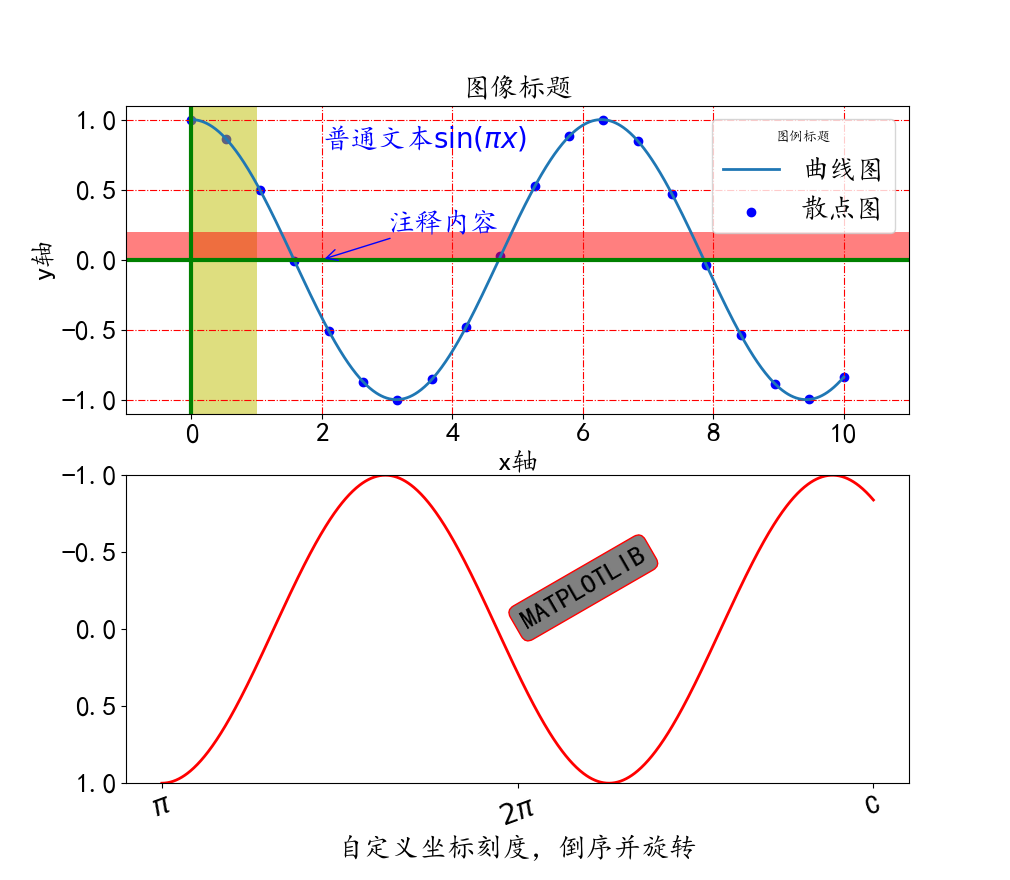
\includegraphics[width=12cm]{./figures/PyPlot_2.png}
\caption{matplotlib库的基本使用} \label{PyPlot_fig2}
\end{figure}

\begin{enumerate}
\item 代码1-3行先导入需要使用的python库
\item 5-6行对字体进行设置,默认情况下中文不显示
\item 7行在一个画布上面划分两行一列的区域,并将后续作图显示在第一个区域
\item 8-11行产生xy数据
\item 12,13行分别绘制曲线图与散点图, \verb|ls| 是 \verb|linestyle| 缩写, \verb|lw|是 \verb|linewidth| 缩写, \verb|c| 是 \verb|color|, \verb|label| 是图例名称
\item 15-19行分别限制坐标轴范围,设置坐标轴名称,已经添加网格线操作.
\item 后续代码,相关说明可以看源码注释部分
\end{enumerate}

